Previous work demonstrated that applying electric fields to silica-stabilized emulsion droplets 
caused particle stabilizers to unjam and then rejam, locking the emulsion in a new morphology. 
\cite{cui_stabilizing_2013} Considering the potential applications of an already synthesized porous 
material with tunable microstructure, the second part of this work will explore using magnetic fields 
to manipulate bijels after synthesis. \cite{vanoli_bijels_2022, cha_bicontinuous_2019} Bijels simulated 
under no field had a constant magnetic in the z direction of strength $\Bar{B} = 0, 0.2, 0.5, 1$ with their
 microstructure and particle order analyzed.

Underlying mechanism being rearrangement of particles on the interface in response to magnetic field, or 
unjamming and rejamming characterized by a change in the number of bonded neighbors. Explains behaviour 
seen in differences in the system above and below the isotropic to nematic transition? 

\begin{figure}
    \centering
    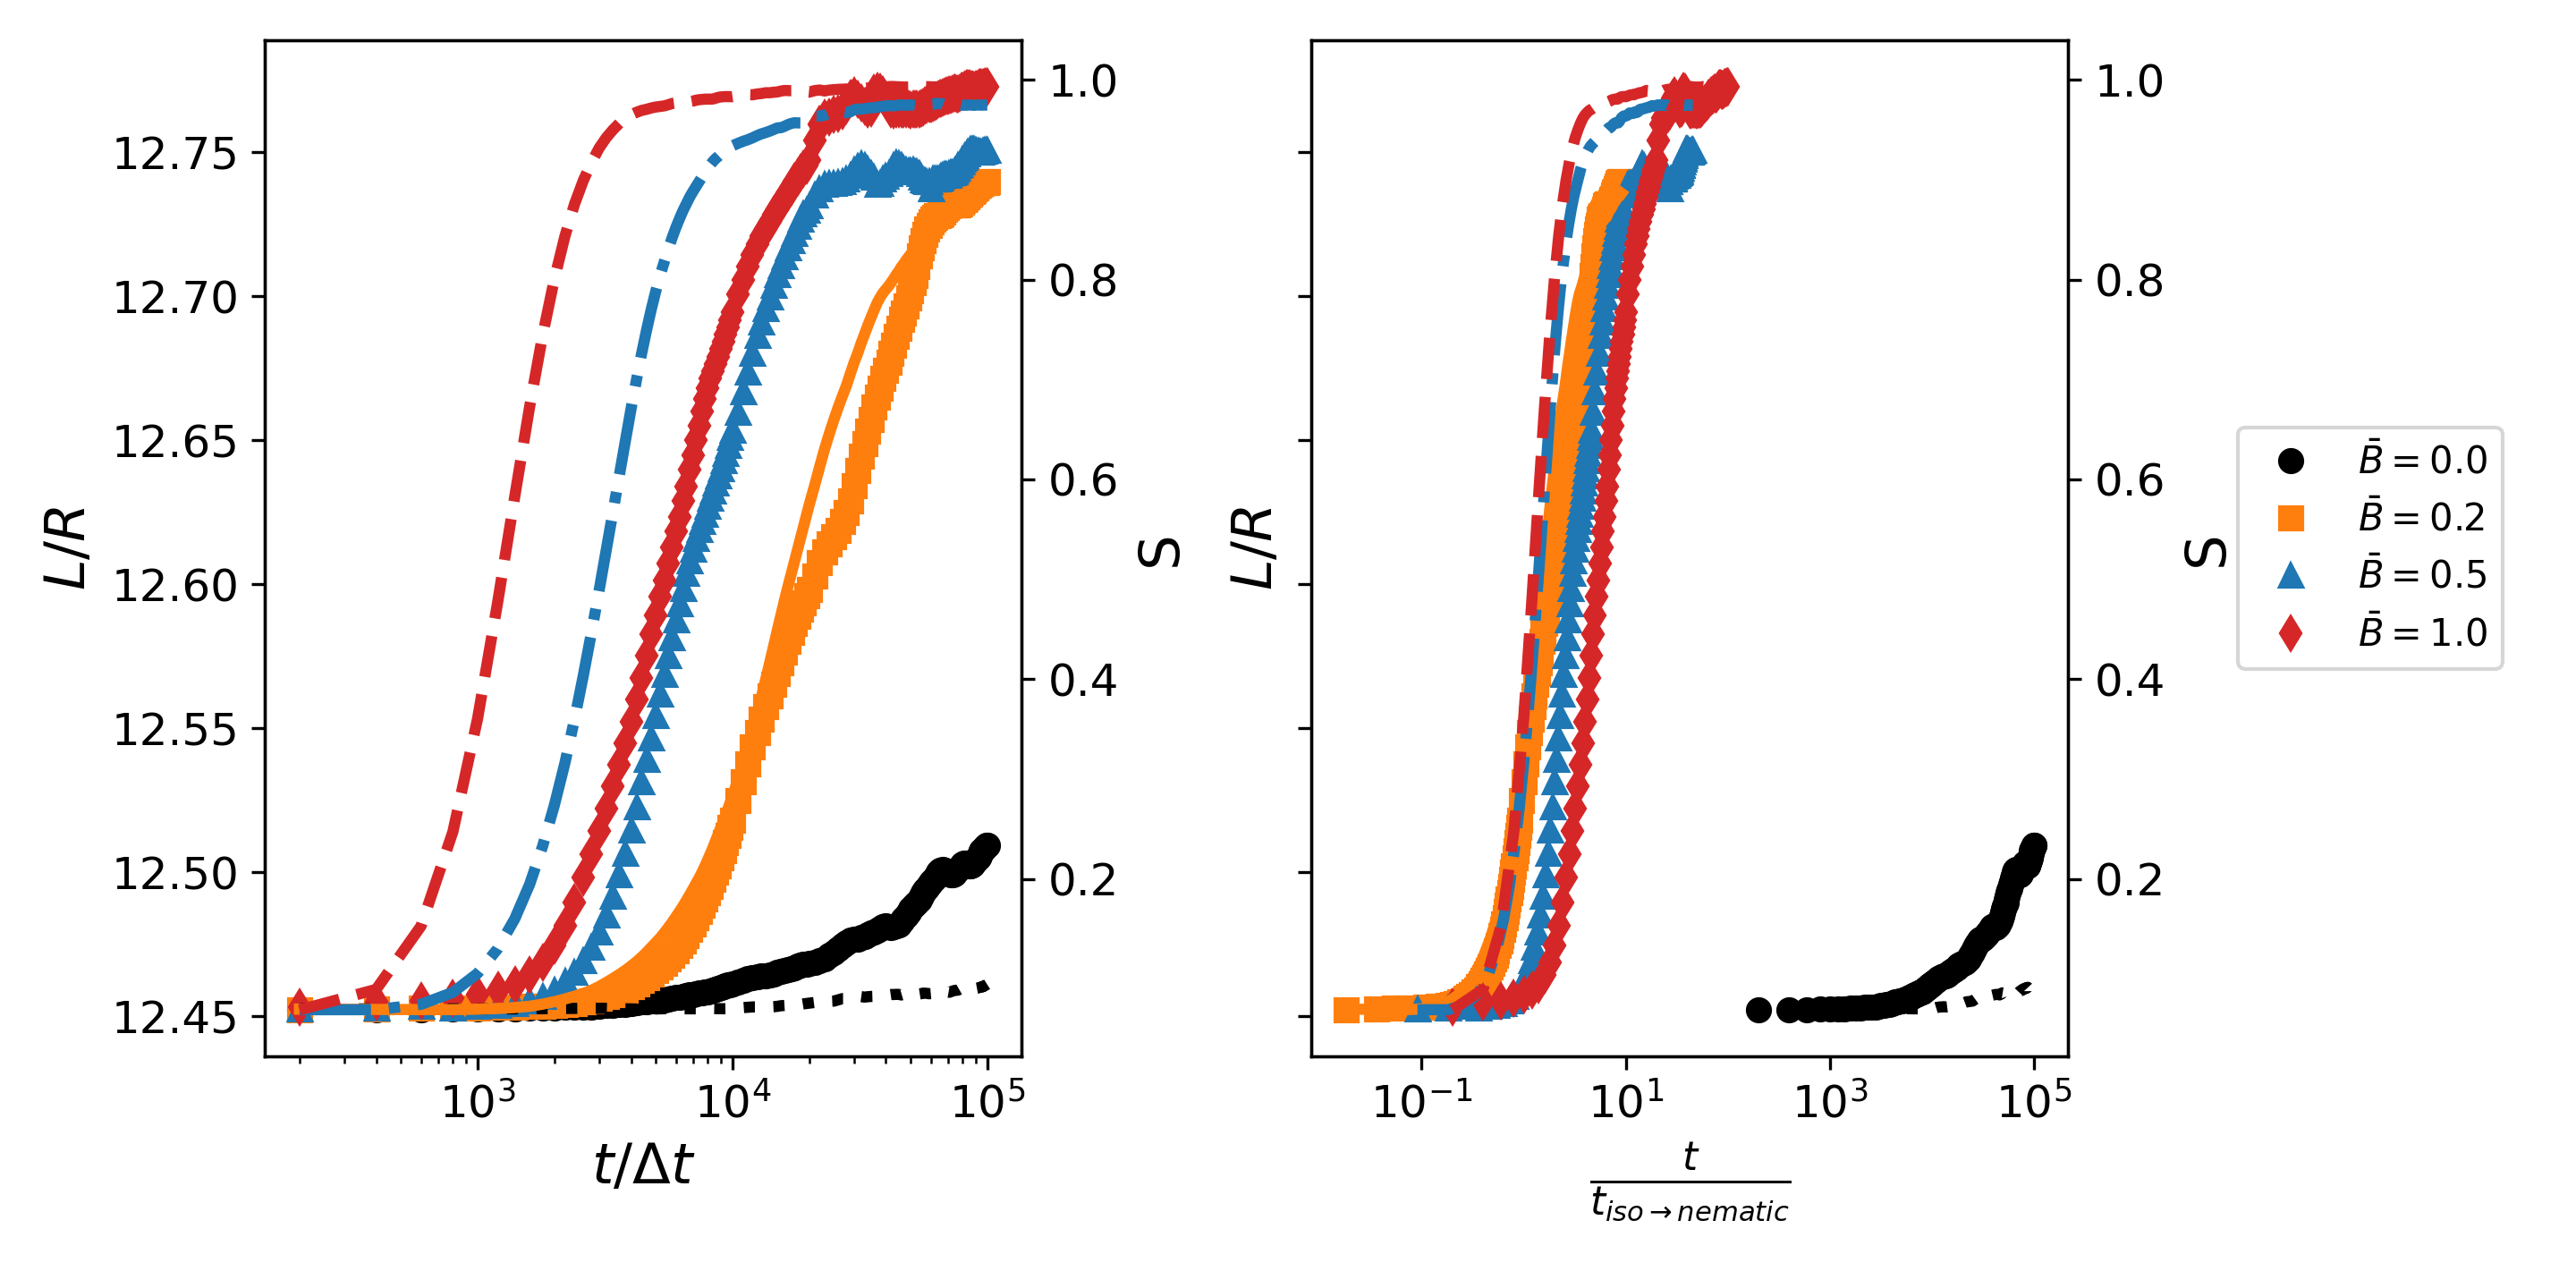
\includegraphics[scale = 0.5]{figures/results/paper2/domain_size.png}
    \caption{Left plot shows the average domain size $(L_1)$ in markers and the nematic order parameter $(S)$ in lines versus time. Right plot shows the same data rescaled over $t_{iso \rightarrow nematic}$.}
    \label{fig:P2_domain_scaling}
\end{figure}

In this system, the mechanism of microstructure modification after formation is expected to be due to magnetic 
field driven particle ordering changes. Figure \ref{fig:P2_domain_scaling} demonstrates that the average domain 
size $(L_1)$ does not change significantly with the applied field, with a slight increase of about $\approx 0.3 L/R$, 
noted to be within error. However, clues into the underlying mechanics are visible when examining the nematic order 
parameter lines overlaid on the domain size markers. At $\Bar{B} = 0.2$, the domain size change corresponds with the 
nematic order parameter change, indicating a direct link between domain size change and particle ordering. 
At $\Bar{B} > 0.2$, a gap appears between the domain size change and the nematic order parameter change, suggesting 
steric effects influence the rate of bijel microstructure change. The timescales of these rearrangements may also 
impact the observed microstructure changes, which can be characterized by the domain size change over time rescaled 
by a characteristic timescale.

A naive guess as to the dominating timescale of the response would be the isotropic to nematic time of the 
system or when $S \geq 0.3$. The right plot of Figure \ref{fig:P2_domain_scaling} demonstrates the time 
evolution of the system when rescaling time with the isotropic to nematic transition time,
 $t_{iso \rightarrow nematic}$. From this plot, it can be seen that application of the field 
 causes collapse of domain size changes at different field strengths on top of one another, 
 showing that this naive guess is a correct one. The changes in domain size at with no applied
  field can be attributed to the reordering of particles at the interface, leading to coarsening 
  at long time scales consistent with what Gunther et al. observed. \cite{gunther_timescales_2014}

\begin{figure}
    \centering
    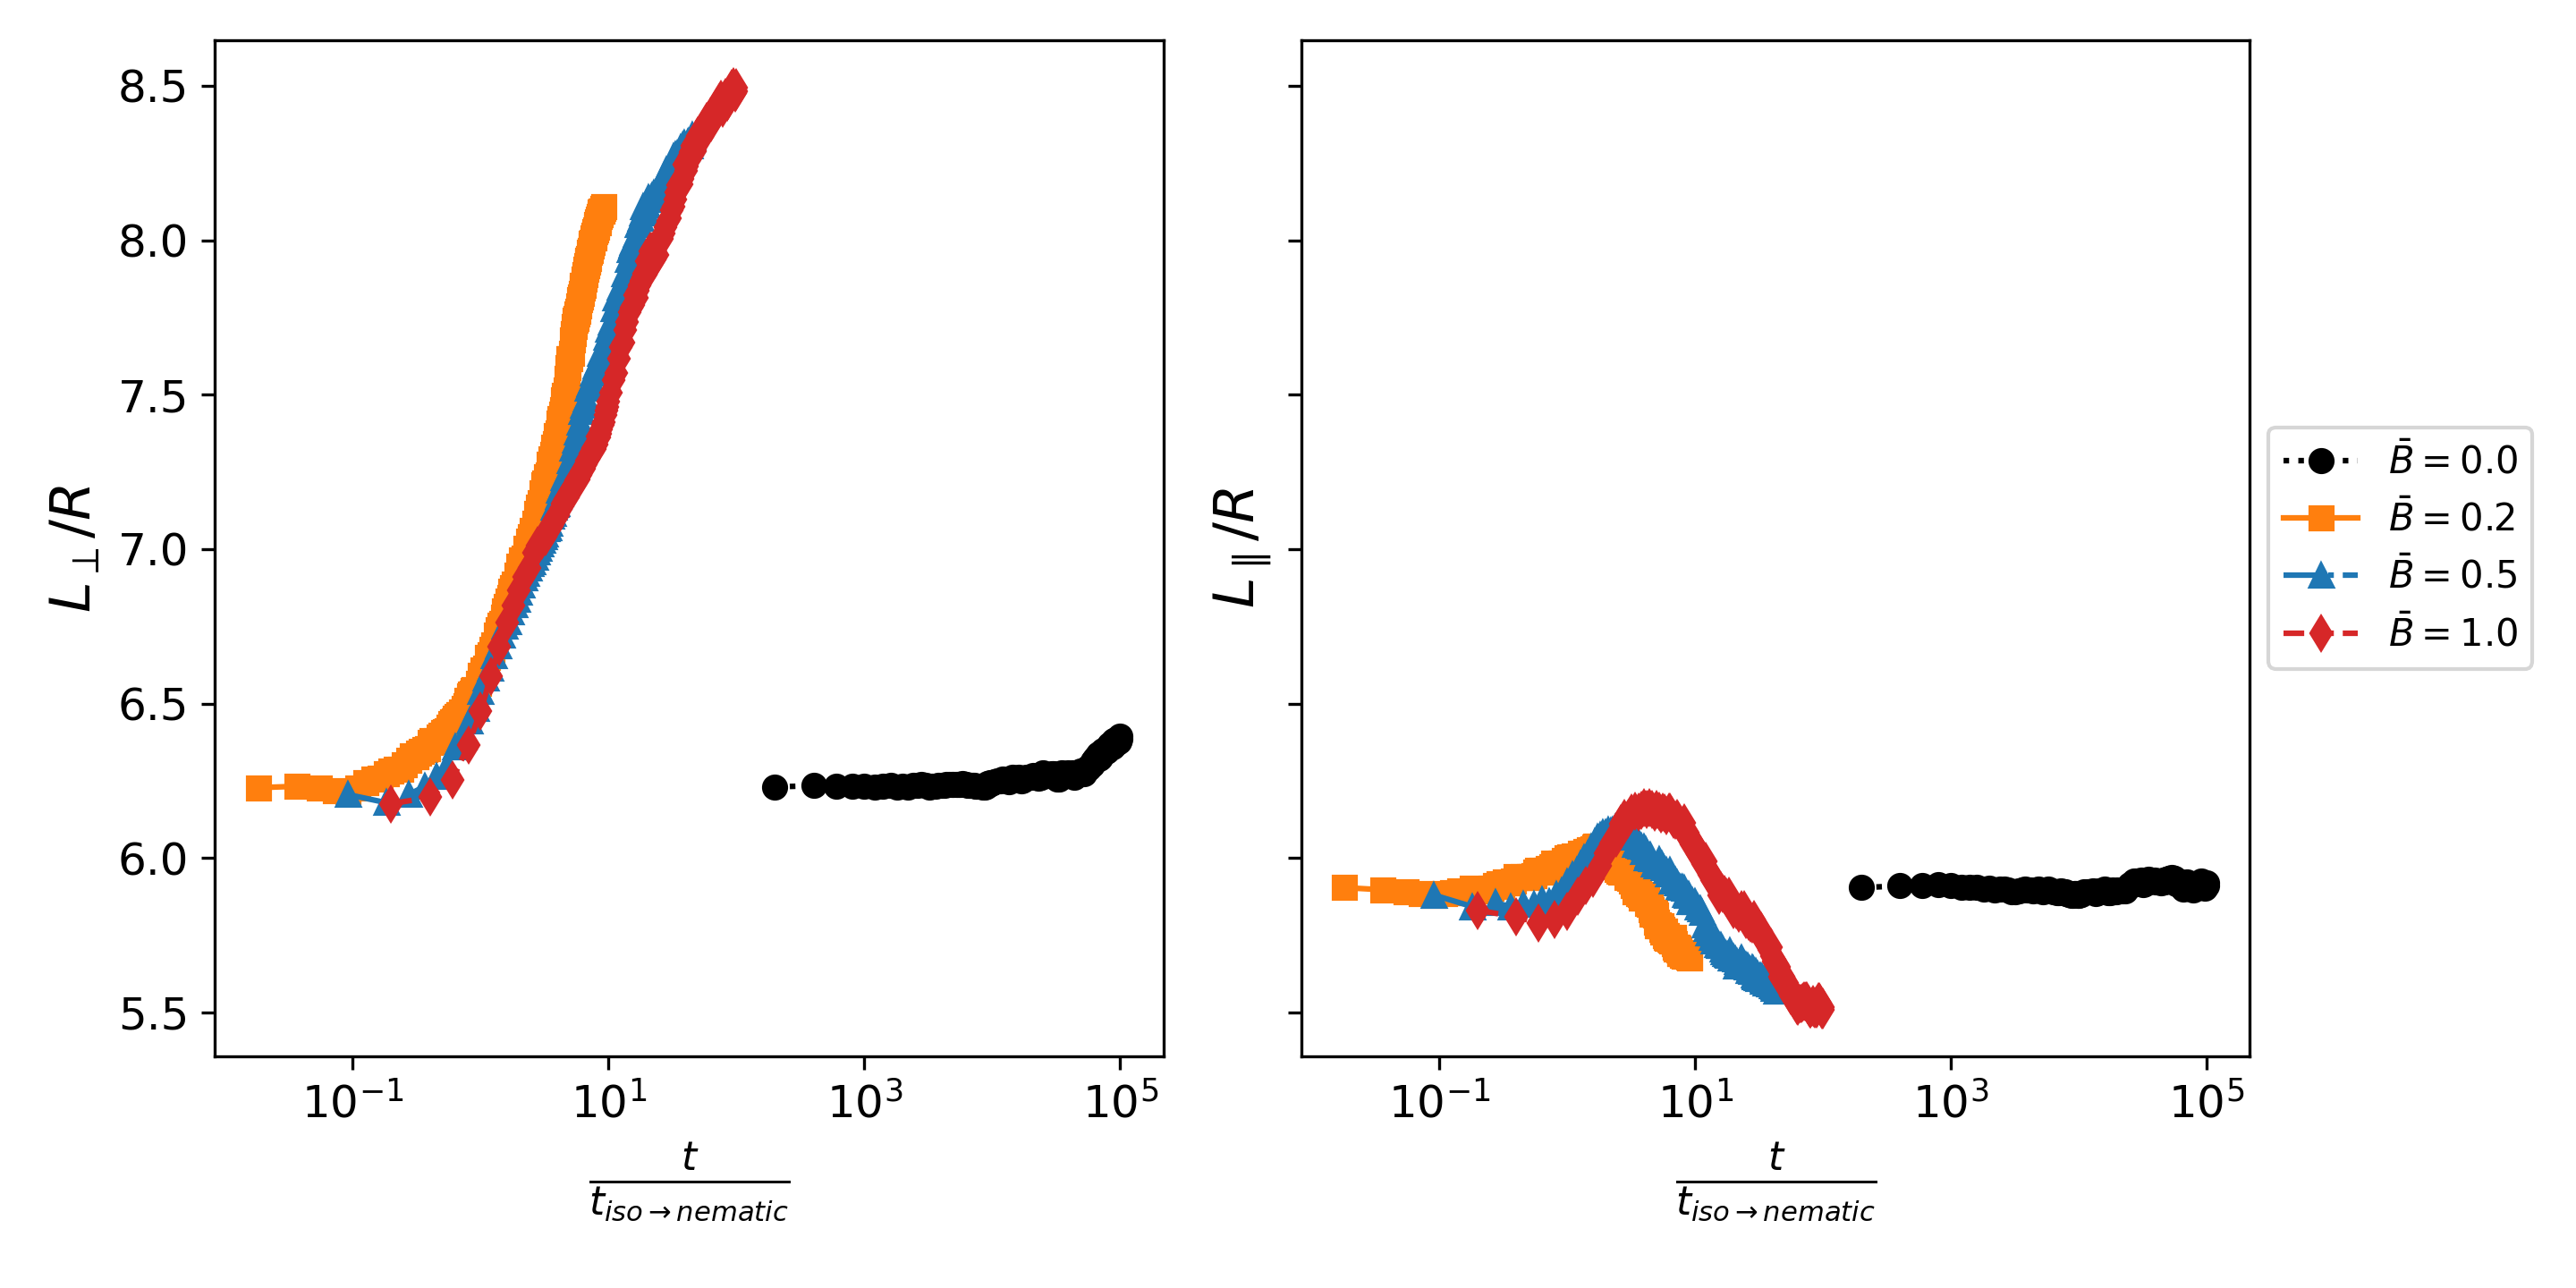
\includegraphics[scale = 0.5]{figures/results/paper2/domain_size_aniso.png}
    \caption{Plots of the perpendicular $(L_{\perp})$ and parallel $(L_{\parallel})$ domain sizes over time rescaled over $t_{iso \rightarrow nematic}$}
    \label{fig:P2_domain_aniso}
\end{figure}

In the previous section, even if the average domain size did not change much, there was domain size anisotropy 
found upon application of the field. This observation and trends seen remains true when applying the field 
after formation as can be observed in \ref{fig:P2_domain_aniso}. Time was again rescaled with the isotropic 
to nematic transition time for each system, demonstrating that the timescale of response is controlled using 
this timescale, and is independent from field strength. The domain size change observed appears to be about $1 L/R$ 
less than what can be found when applying the same field size during bijel synthesis as the increase in domain size 
for $L_{parallel}$ for prolate particles is $\approx 2 L/R$ which is $50 \%$ lower than what was found. This 
indicates that microstructure control after synthesis is not as effective. This might be due to steric effects 
being much stronger after synthesis, limiting how much particles can move or tilt before rejamming. Despite 
this, the domain size change found is well within what has been seen to be effective in the literature, 
indicating that magnetic field enabled in-situ microstructure modifications can be utilized within bijels. 
\cite{cha_bicontinuous_2019, khan_nanostructured_2022, vanoli_bijels_2022}

\begin{figure}
    \centering
    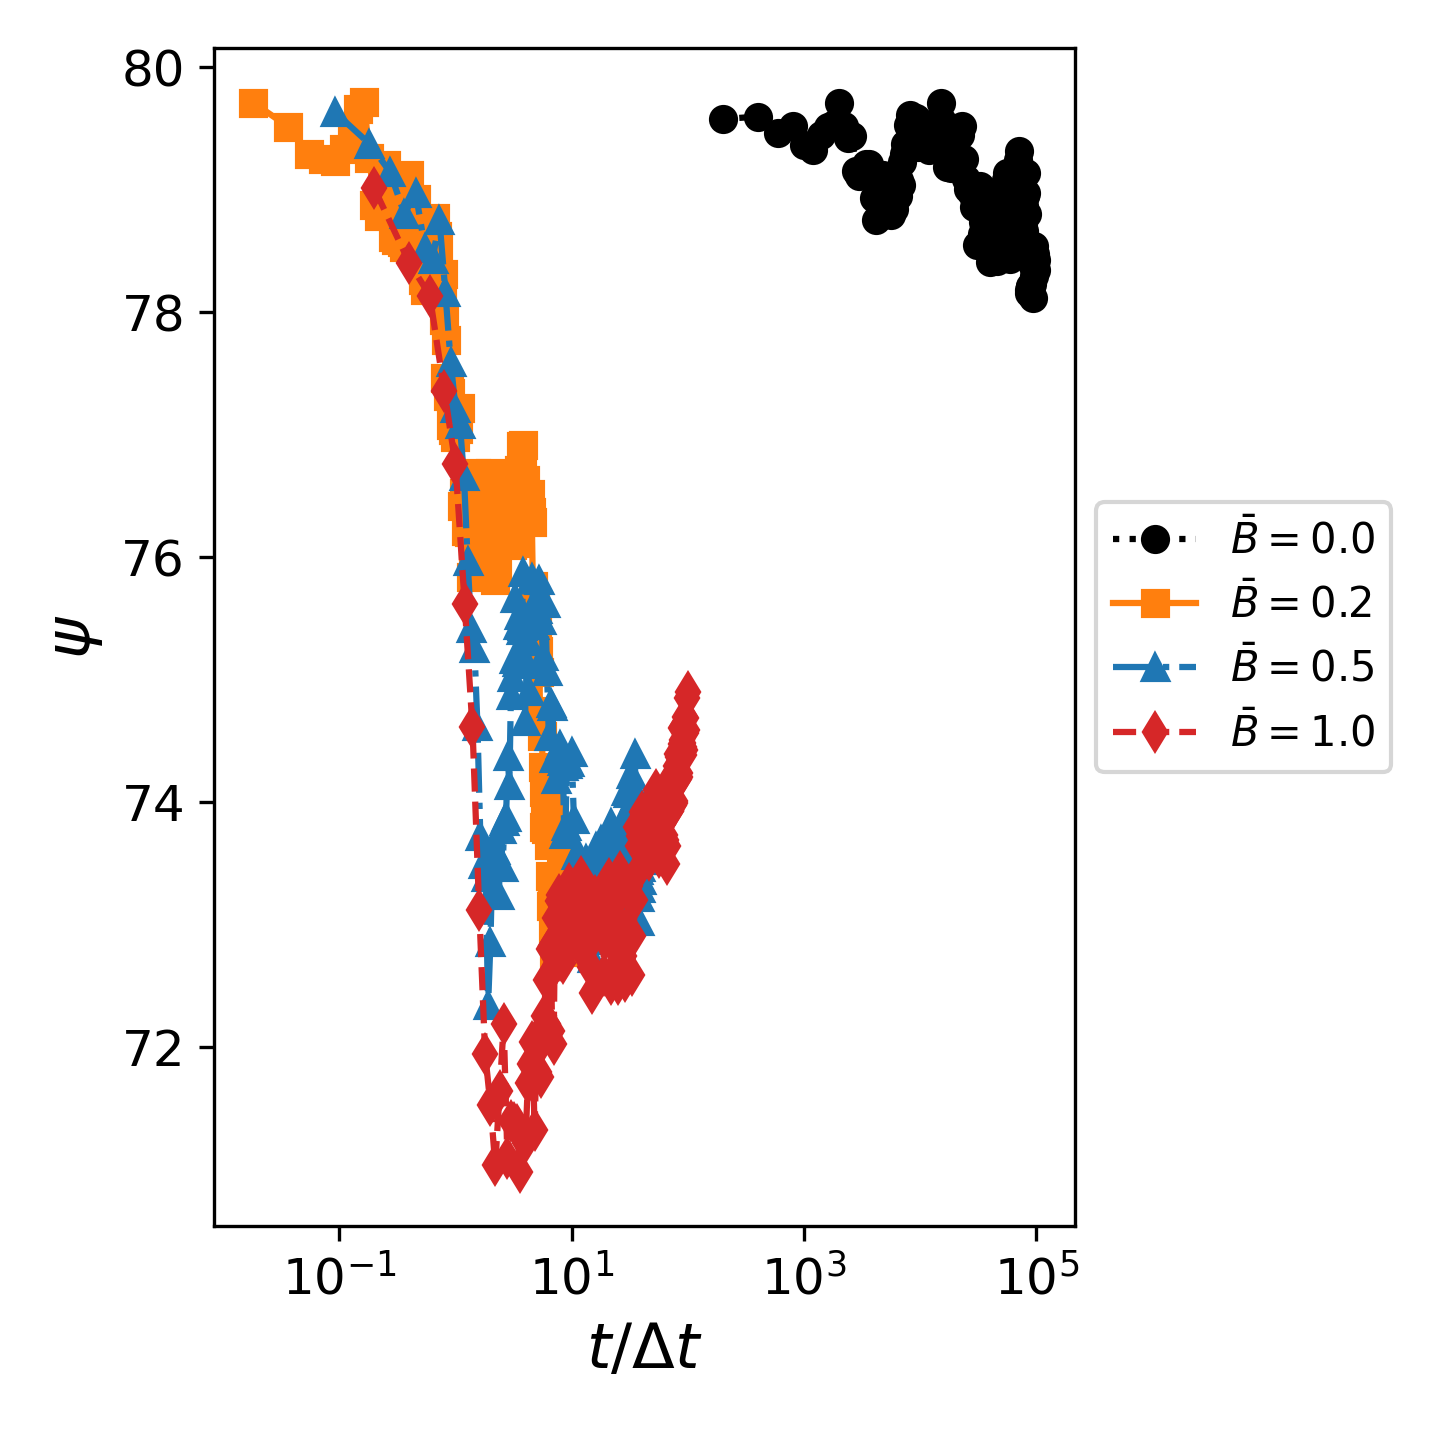
\includegraphics[scale = 0.5]{figures/results/paper2/interface_angle.png}
    \caption{Plots of the average angle between the particle dipole moment and interface normal $(\psi)$ over time. While there are minor changes in for the oblate particles, these are not as significant as the ordering of particles to the field.}
    \label{fig:P2_interface_angle}
\end{figure}

To determine if the interface follows the orientation of the particles, the average angle between the 
particle symmetry axis and the interface normal $(\psi)$ was plotted against time rescaled by 
$t_{iso \rightarrow nematic}$ in Figure \ref{fig:P2_interface_angle}. From ths plot, it can be 
observed that upon application of the magnetic field, the particle tilts out of the interface at 
an equal normalized rate. However, the angle reached before the particles begin returning to their 
equilibrium configuration is magnetic field strength dependent, suggesting that the degree of 
microstructure changed observed might be dependent on how much the particle tilts away from its 
equilibrium position. At non-equilibrium particle tilts, there is more leeway for coarsening to 
occur before rejamming occurs, resulting in larger microstructural differences. 

Future work will more closely examine the role of the particles in observed microstructure changes 
by calculating the average angle between the particle symmetry axis and the interface normal. 
In addition, the impact of initial order of the particle monolayer on the degree of microstructure 
change observed will be characterized. This will be accomplished by using bijels that have been 
simulated under magnetic fields and changing the applied field. Example conditions would be a bijel 
being simulated under a field strength of $\Bar{B} = 0.2$ and increasing the applied field to $\Bar{B} = 1$ 
or switching off the applied field. Based on the findings so far it is predicted that initial particle order 
and microstructure change are inversely correlated. Additionally, the timescales of these microstructure 
changes will be investigated. When switching a field on, there are magnetic field, steric and interfacial 
forces that govern the dynamics. However, when reducing the field strength, the magnetic field derived force 
isn't present, resulting in steric and interfacial forces playing a significant role. These differences can 
be examined by investigating the timescales the observed response occurs at, as well as the particle 
properties over time.

% \textcolor{blue}{Still needs additional explanation of how using templates made under fields and decreasing and increasing field strengths will change results}
